%-------------------------------------------------------
\section{Clustering}
%-------------------------------------------------------

\begin{frame}{Cluster Analysis}{How can we find semantic groups among data instances?}

 \centering\textit{Obtaining a clustering on the joined data set:} \vspace{0,3cm}

	\begin{block}{}
		\begin{itemize}
			\item<1-> \alert{K-Means} --- others algorithms as been tried, but K-Means gave the best results;
			\item<2-> \alert{2 clusters} --- deviding teaching courses in \emph{good} ones and \emph{not-so-good} ones;
			\item<3-> \alert{3 attributes} --- each one express a fundamental aspect of the whole data set: \emph{average exam score, average teaching evaluation} and \emph{average delay}.
		\end{itemize}
	\end{block}

\end{frame}

\begin{frame}{Cluster Analysis}{How can we find semantic groups among data instances?}

    \textbf{X axis}: \emph{average delay} \\ \textbf{Y axis}: \emph{average exams mark}

    \vspace{0.1cm}
    \begin{centering}
        \hspace{0.5cm}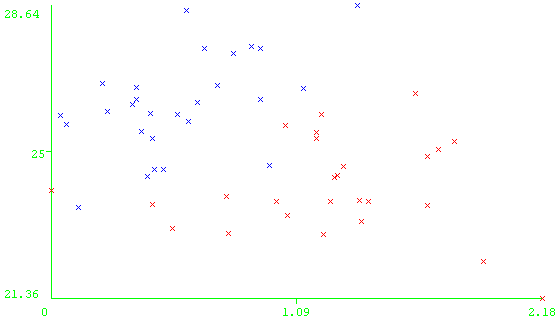
\includegraphics[scale=0.46]{cluster1.png}
    \end{centering}

    \textcolor{blue}{Cluster 0}: good courses --- \textcolor{red}{Cluster 1}: bad courses

\end{frame}

\begin{frame}{Cluster Analysis}{How can we find semantic groups among data instances?}

\textbf{X axis}: \emph{average delay} \\ \textbf{Y axis}: \emph{average teaching evaluation}

    \vspace{0.1cm}
    \begin{centering}
        \hspace{0.5cm}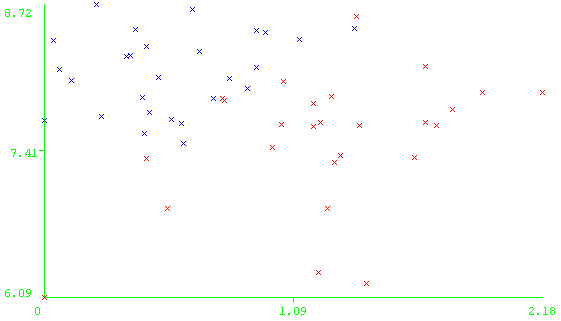
\includegraphics[scale=0.46]{cluster2.png}
    \end{centering}

    \textcolor{blue}{Cluster 0}: good courses --- \textcolor{red}{Cluster 1}: bad courses

\end{frame}

\begin{frame}{Cluster Analysis}{How can we find semantic groups among data instances?}

\textbf{X axis}: \emph{average exams mark} \\ \textbf{Y axis}: \emph{average teaching evaluation}

    \vspace{0.1cm}
    \begin{centering}
        \hspace{0.5cm}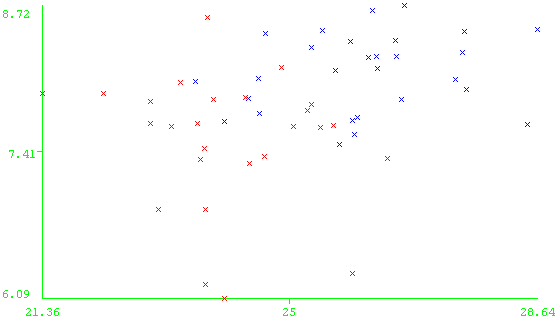
\includegraphics[scale=0.46]{cluster3.png}
    \end{centering}

    \textcolor{blue}{Cluster 0}: good courses --- \textcolor{red}{Cluster 1}: bad courses

\end{frame}

\begin{frame}{Cluster Analysis}{How can we find semantic groups among data instances?}

    Sum of the \emph{average delay} of each instance, for each Academical Year and for each cluster

    \begin{centering}
        \hspace{0.5cm}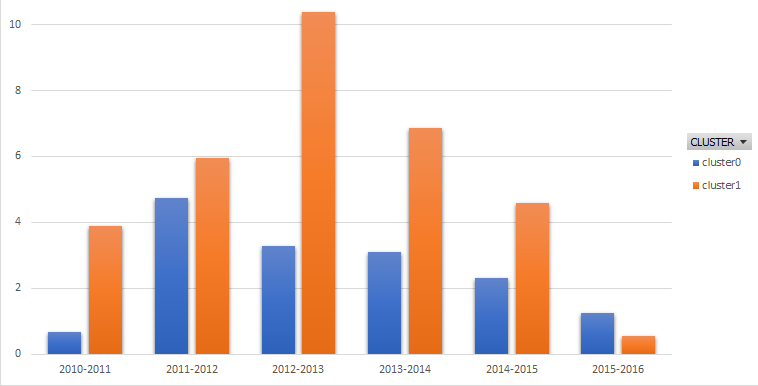
\includegraphics[scale=0.40]{cluster4.png}
    \end{centering}

\end{frame}

\begin{frame}{Cluster Analysis}{How can we find semantic groups among data instances?}

    corsi unicamente nei clsuter, senza contare l'anno

    \begin{centering}
        \hspace{0.5cm}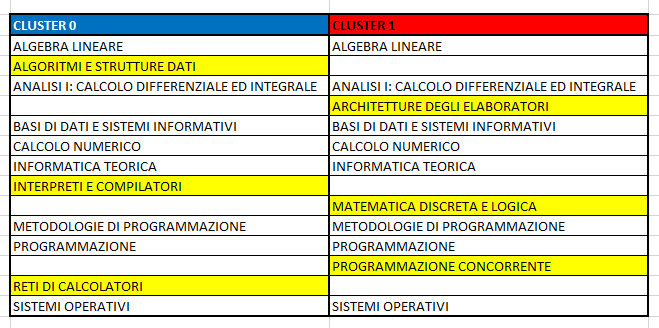
\includegraphics[scale=0.40]{../cluster/min_kmeans_2cl_corsi_cluster.png}
    \end{centering}

\end{frame}